A monophase, steady and fully developed flow of a Newtonian 
and incompressible fluid between parallel and fixed horizontal 
plates is maintained due to a pressure gradient 
$\partial p/ \partial x$ imposed as mentioned by Pontes 
and Mangiavacchi (2016) \cite{pontes2016}. 
This flow is known as \textit{Poiseuille flow}. 
The \ref{poiseuille} presents schematically this flow and 
the expected velocity field.

\begin{figure}[H]
\caption{Poiseuille Flow}
\begin{center}
\begin{tikzpicture}[scale=1.3]
 \draw [pattern=north east lines] (0,0) -- (0,-0.1) -- (5,-0.1) -- (5,0) -- cycle;
 \draw [pattern=north east lines] (0,1) -- (0,1.1) -- (5,1.1) -- (5,1) -- cycle;

 \draw [->,thick] (-2,-0.1)--(-2,1.5) node[left] {$y$};
 \draw [->,thick] (-2.1,0)--(-0.5,0) node[below] {$x$};
 
 \draw [dotted] (2.5,0.0) to (2.5,1.0);
 \draw  (2.5,0.0) to [bend right=100] (2.5,1.0);
 
 \draw [->,thick] (2.5,0.9) to (2.7,0.9);
 \draw [->,thick] (2.5,0.7) to (2.78,0.7);
 \draw [->,thick] (2.5,0.5) to (2.8,0.5);
 \draw [->,thick] (2.5,0.3) to (2.78,0.3);
 \draw [->,thick] (2.5,0.1) to (2.7,0.1);
\end{tikzpicture}
\end{center}
\label{poiseuille}
\end{figure}

\noindent
The velocity profile equation is shown below:

\begin{equation}
 u = \frac{4 u_{max}}{L^2} y \big[ L - y \big]
\end{equation}

\medskip
\noindent
where $u_{max}$ is maximum velocity and its value is 
$u_{max} = 1.5$, $L$ is non-dimensional length 
between the plates and its value is 
$L = 1$
and $y$ is the vertical coordinates and it varies 
between $y = \big[ 0,1 \big]$.
The domain was discretized using a linear triangular mesh
with 3835 nodes and 7299 elements.
The \ref{velocidade poiseuille} shows the steady state velocity profile
when $Re=100$.
It is possible to observe that the numerical
solution converges to the analytical solution.

\vspace{1cm}
\begin{figure}[H]
     \caption{
Steady state velocity profile when $Re=100$ and the comparison between
the numerical and analytical solution for Poiseuille flow.} 
     \centering
     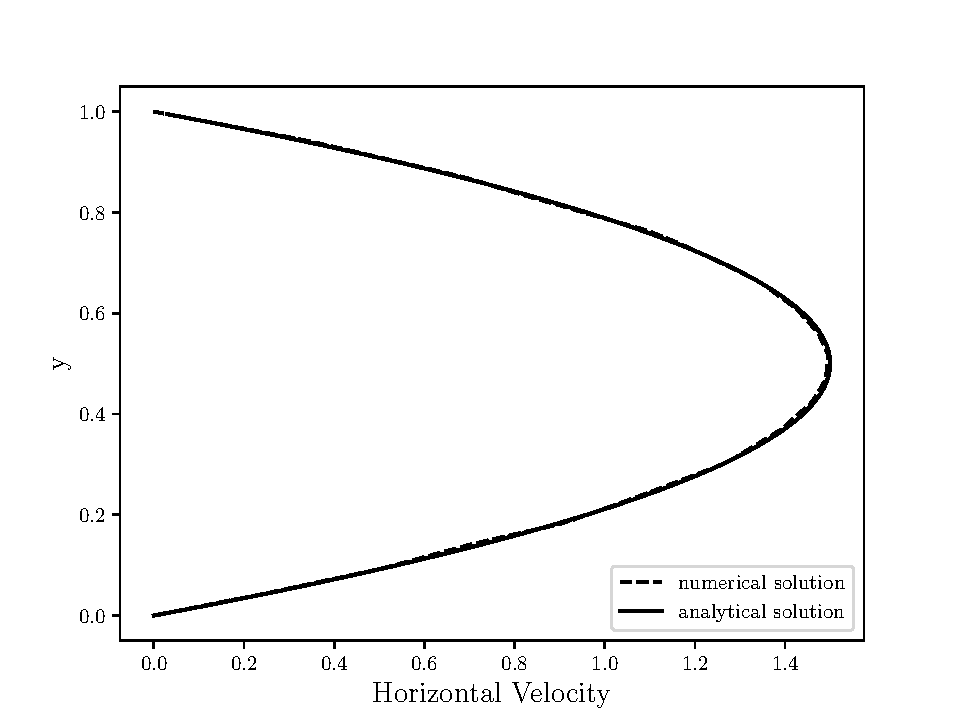
\includegraphics[scale=1]{./02_chaps/cap_validation/figure/poiseuille_velocity.pdf}\\
     \medskip
     \label{velocidade poiseuille}
\end{figure}

\newpage
The \ref{erro relativo poiseuille tabela} shows the relative error 
between the numerical solution and the analytical solution 
for several unstructured linear triangular meshes, ranging 
from 100 to 25600 linear triangular elements. For the mesh 
with 7299 elements as in the case of this benchmark problem, 
the estimated relative error for the velocity field is 0.4\%.

\vspace{0.5cm}
\begin{table}[H]
\centering
\begin{tabular}{ccc}
\toprule
\textbf{Elements} & \textbf{Error} (\%) \\
\midrule
100 & 25.00 \\
400 & 7.47 \\
1600 & 2.11 \\
6400 & 0.61 \\
25600 & 0.17 \\
\bottomrule
\end{tabular}
\caption{The relative error of numerical solution for several elements numbers in an unstructured linear triangular mesh.}
\label{erro relativo poiseuille tabela}
\end{table}

\noindent
\medskip
The relative error was estimated as:

\begin{equation}
 \mathit{Error} = \sqrt{\frac{\sum{(v_{n} - v_{a})^{2} }}{\sum |v_{a}|^{2} }}
\end{equation}

\noindent
where $v_{n}$ is the numerical velocity fielf and
$v_{a}$ is the analytical velocity field.

\bigskip
The \ref{ordem de convergencia poiseuille} presents the relative error 
of the numerical solution with the first and second order convergence 
curves on a log-log scale. As can be seen, the relative error of 
the numerical solution for Poiseuille flow has the form of 
first order convergence. Thus, when increasing the number of elements, 
the relative error of the numerical solution regresses linearly.
A possible cause is due to the vorticity boundary condition used 
in this work. Therefore, the use of the 2a-order boundary condition
would possibly improve the order convergence of the numerical
solution. However, it is necessary to be investigated. 


\begin{figure}[H]
     \caption{Convergence order in log-log scale:
It is estimated the the relative error of numerical solution has
first order convergence.}
     \centering
     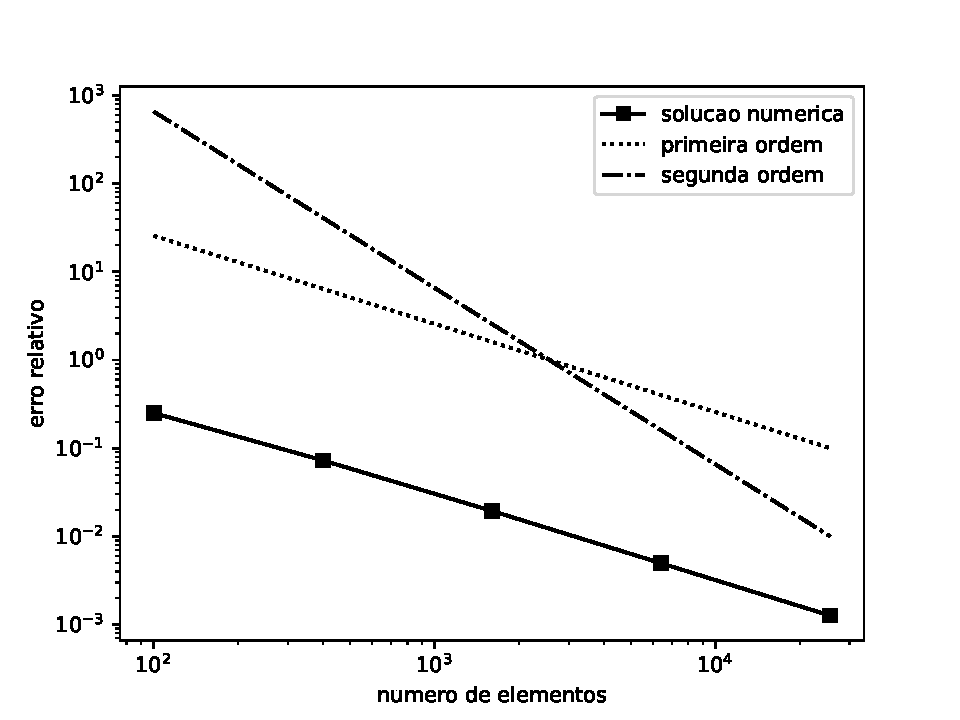
\includegraphics[scale=1]{./02_chaps/cap_validation/figure/poiseuille_error.pdf}\\
     \medskip
     \label{ordem de convergencia poiseuille}
\end{figure}


